\section{Resultados}
\label{sec:results}

O método proposto na seção~\ref{sec:metodo} foi implementado na linguagem \textit{C++} para um melhor desempenho, e também possibilitar uma comparação mais justa com os \textit{baselines}, os quais também foram todos implementados em \textit{C++}. 

\subsection{Configuração dos experimentos}
\label{sec:experiments-setup}
Nos experimentos são comparados os seguintes algoritmos:
\begin{itemize}
    \item ICAN \citep{ji2009efficient}
    \item ICPAN \citep{li2011efficient}
    \item META \citep{deng2016meta}
    \item IP2L -- Uma variação do método apresentado na seção~\ref{sec:metodo} que processa todos os nós pivô ativos com busca sequencial, sem utilizar a busca binária.
    \item IP2LB -- Método apresentado na seção~\ref{sec:metodo} na íntegra.
\end{itemize}

Os resultados de tempo processamento do META não serão considerados na exibição dos gráficos de linha, pois seus valores são muito maiores, o que dificulta a visualização dos gráficos. Além disso, todos os códigos-fonte dos \textit{baselines} são os originais utilizados pelos autores de seus respectivos artigos.

Todos os experimentos foram realizados em uma máquina de servidor com processador \textit{Intel \textsuperscript{\textregistered} Xeon E5 4617 2.90 GHz}, com \textit{64GB} de memória \textit{RAM}, tendo o \textit{Ubuntu 18.04.1 LTS} como sistema operacional. Os algoritmos foram compilados com o \textit{gcc 7.4.0}. Os experimentos aqui apresentados servem para provar o conceito do método proposto neste trabalho, mas planejamos ainda realizar um novo conjunto de experimentos mais robustos e detalhados para concluir a pesquisa.

Utilizamos uma base de dados pública denominada \textit{USADDR}, a qual é um conjunto com $10$ milhões de endereços e localizações dos Estados Unidos da América, extraídos da coleção \textit{SimpleGEO CC0}. Dessa base, os itens foram extraídos e inseridos em um único arquivo de texto no qual cada linha representa um item. Nela há um total de $10.251.121$ itens e $32.407.449$ palavras com tamanho médio igual a $6,249$ caracteres. Cada item possui uma média de $3,161$ palavras e tamanho médio médio igual a $19,757$ caracteres.

Todos os experimentos para medir o tempo de processamento foram realizados com uma média de $50$ consultas extraídas aleatoriamente da base de dados, com tamanhos variando de $3$ a $13$ (aumentando de $2$ em $2$), considerando $\tau=3$. Todas essas consultas tiveram seu terceiro caractere modificado por um novo diferente do atual, representando um erro de substituição. Para cada execução de cada algoritmo, também foi medido seu pico de memória utilizado.

\subsection{Tempo de processamento do método IP2LB}

A Tabela~\ref{tab:metodo-performance} apresenta a média de tempos (em $ms$) de processamento de consultas de prefixo $q$ utilizando o método IP2LB. A primeira coluna ``carac.'' representa os valores de $\lambda$ variando de $4$ até $10$, e as próximas colunas contêm as médias de tempo de processamento para cada tamanho $|q|$ de consulta. Para cada valor de $\lambda$ foram realizadas $50$ consultas como descrito na seção~\ref{sec:experiments-setup}, pois na prática cada valor de $\lambda$ para o método IP2LB (e IP2L) produz um modelo por si só, denominado IP2LB-$\lambda$.

\begin{table}[h]
\centering
\begin{tabular}{c|c|c|c|c|c|c|}
\cline{2-7}
 & \multicolumn{6}{c|}{\textbf{Tamanho do Prefixo Consultado}} \\ \hline
\multicolumn{1}{|c|}{\textbf{carac.}} & \textbf{|q| = 3} & \textbf{|q| = 5} & \textbf{|q| = 7} & \textbf{|q| = 9} & \textbf{|q| = 11} & \textbf{|q| = 13} \\ \hline
\multicolumn{1}{|c|}{4} & 104.414 & 225.847 & 255.190 & 262.910 & 273.861 & 263.856 \\ \hline
\multicolumn{1}{|c|}{5} & 116.767 & 58.892 & 117.848 & 117.092 & 124.004 & 129.742 \\ \hline
\multicolumn{1}{|c|}{6} & 118.174 & 67.707 & 83.576 & 85.318 & 90.690 & 92.876 \\ \hline
\multicolumn{1}{|c|}{7} & 123.378 & 71.812 & 71.817 & 79.232 & 82.692 & 85.913 \\ \hline
\multicolumn{1}{|c|}{8} & 122.283 & 74.391 & 75.281 & 78.995 & 82.135 & 84.005 \\ \hline
\multicolumn{1}{|c|}{9} & 125.307 & 76.704 & 78.162 & 77.523 & 83.250 & 83.335 \\ \hline
\multicolumn{1}{|c|}{10} & 120.886 & 77.993 & 80.702 & 79.195 & 85.414 & 119.491 \\ \hline
\end{tabular}
\caption{Tempos de processamento em $ms$ para o método IP2LB variando o tamanho do prefixo de consulta $q$ e variando também o $\lambda$ (coluna ``carac.''), a altura máxima para a \textit{trie}.}
\label{tab:metodo-performance}
\end{table}

Na Figura~\ref{fig:varying-usaddr-tau-3} estão representados os resultados da Tabela~\ref{tab:metodo-performance}. Há $7$ curvas (uma para cada valor de $\lambda$) de tempo de processamento em função do tamanho da consulta, para o método IP2LB variando o tamanho do prefixo de consulta $q$ e variando também o $\lambda$, a altura máxima para a \textit{trie}. 

\begin{figure}[ht!]
    \centering
    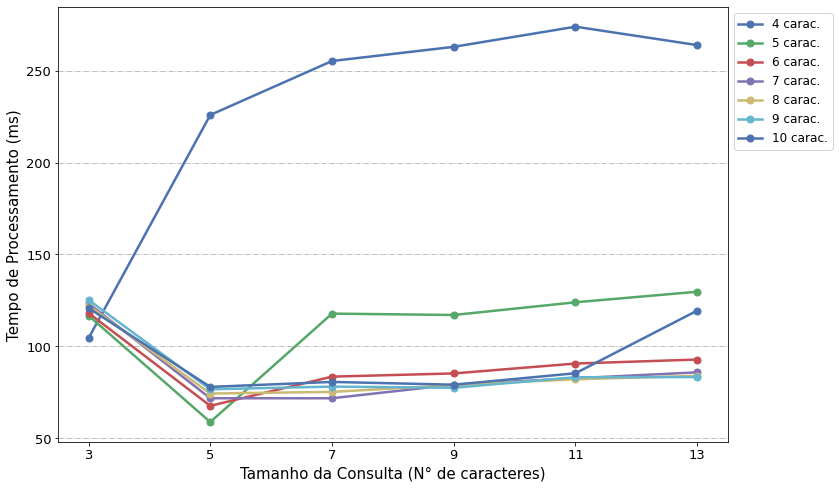
\includegraphics[width=0.95\textwidth]{figures/varying_trie_prefix_method_IP2LB_dataset_usaddr_tau_3.png}
    \caption{Curvas de tempo de processamento em $ms$ para o método IP2LB variando o tamanho do prefixo de consulta $q$ e variando também o $\lambda$, a altura máxima para a \textit{trie}.}
    \label{fig:varying-usaddr-tau-3}
\end{figure}

É esperado que, quanto maior for o valor de $\lambda$, menor será o tempo de processamento. Essa tendência pode ser observado no gráfico da Figura~\ref{fig:varying-usaddr-tau-3}. No entanto, para $\lambda = 4$ a sua curva de tempos se distancia bastante das demais. Isso provavelmente ocorre porque, dada a natureza do algoritmo ICPAN, no término do primeiro nível há uma grande quantidade de nós ativos quando se indexa somente os $4$ primeiros caracteres na \textit{trie} (mesmo com sua otimização de poda de nós ativos redundantes).

\subsection{Uso de memória do método IP2LB}

A Tabela~\ref{tab:memory-usage-usaddr-tau-3} exibe a quantidade memória utilizada pelo método IP2LB (segunda coluna) para cada valor de $\lambda$ (primeira coluna).

\begin{table}[!ht]
\centering
\begin{tabular}{|c|c|}
\hline
\textbf{carac.} & \textbf{Memória Utilizada (MB)} \\ \hline
4 & 1378.490 \\ \hline
5 & 1408.363 \\ \hline
6 & 1528.575 \\ \hline
7 & 1749.214 \\ \hline
8 & 2075.432 \\ \hline
9 & 2520.842 \\ \hline
10 & 3078.759 \\ \hline
\end{tabular}
\caption{Quantidades de memória em \textit{MegaBytes} utilizada para cada valor de $\lambda$ no método IP2LB.}
\label{tab:memory-usage-usaddr-tau-3}
\end{table}

A Figura~\ref{fig:memory-usage-usaddr-tau-3} representa os dados da Tabela~\ref{tab:memory-usage-usaddr-tau-3}, contendo uma curva da quantidade de memória utilizada pelo método IP2LB em função do valor de $\lambda$.

\begin{figure}[!ht]
    \centering
    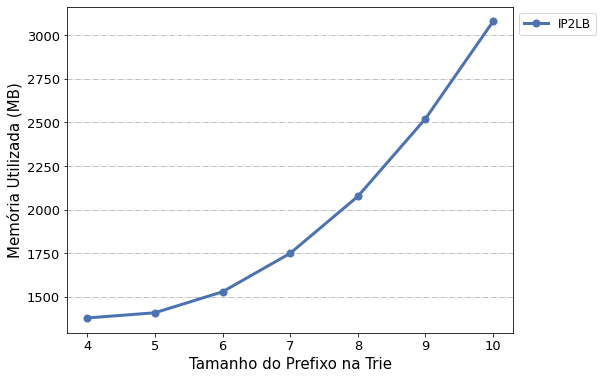
\includegraphics[width=0.95\textwidth]{figures/memory_usage_IP2LB_dataset_usaddr_tau_3.png}
    \caption{Curva de quantidades de memória em \textit{MegaBytes} utilizada para cada valor de $\lambda$ no método IP2LB.}
    \label{fig:memory-usage-usaddr-tau-3}
\end{figure}

É possível observar um padrão exponencial no consumo de memória à medida que a altura máxima permitida para a \textit{trie} aumenta. Isso acontece pois a função do número máximo de nós a cada nível de uma árvore $M-\text{á}ria$ como a \textit{trie} \citep{Knuth:1998} é de fato exponencial com base no tamanho do alfabeto $\Sigma$ considerado. Quanto menos prefixos em comum houver entre os itens indexados, mais o padrão de uso exponencial de memória será atingido.

\subsection{Tempo de processamento de todos os métodos}

A Tabela~\ref{tab:performance-usaddr-tau-3} apresenta as médias de tempo de processamento (em $ms$) para cada método, considerando $\lambda=6$ para IP2LB e o IP2L. Tal valor de $\lambda$ foi escolhido com a intenção de melhor otimizar a relação desempenho/consumo de memória para ambos os métodos. 

\begin{table}[ht]
\centering
\begin{tabular}{c|c|c|c|c|c|c|}
\cline{2-7}
 & \multicolumn{6}{c|}{\textbf{Tamanho da Consulta}} \\ \hline
\multicolumn{1}{|c|}{\textbf{alg.}} & \textbf{|q| = 3} & \textbf{|q| = 5} & \textbf{|q| = 7} & \textbf{|q| = 9} & \textbf{|q| = 11} & \textbf{|q| = 13} \\ \hline
\multicolumn{1}{|c|}{IP2LB-6} & 118.174 & 67.707 & 83.576 & 85.318 & 90.690 & 92.876 \\ \hline
\multicolumn{1}{|c|}{IP2L-6} & 119.540 & 67.749 & 125.885 & 148.891 & 155.325 & 158.376 \\ \hline
\multicolumn{1}{|c|}{ICPAN} & 152.106 & 118.598 & 123.010 & 125.072 & 130.454 & 134.613 \\ \hline
\multicolumn{1}{|c|}{ICAN} & 198.942 & 176.930 & 200.260 & 201.083 & 209.302 & 200.332 \\ \hline
\multicolumn{1}{|c|}{META} & 3180.390 & 5458.480 & 5583.350 & 5794.830 & 6021.520 & 6006.690 \\ \hline
\end{tabular}
\caption{Tempos de processamento em $ms$ dos métodos, considerando $\lambda = 6$ para os métodos IP2LB e IP2L.}
\label{tab:performance-usaddr-tau-3}
\end{table}

A Figura~\ref{tab:performance-usaddr-tau-3} contém uma curva de tempo de processamento em função do tamanho do prefixo de consulta as médias de tempo de processamento (em $ms$) para cada método, considerando $\lambda=6$ para IP2LB e o IP2L.

\begin{figure}[ht]
    \centering
    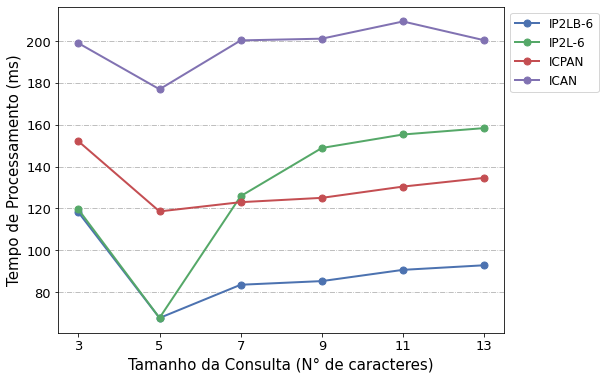
\includegraphics[width=0.9\textwidth]{figures/performance_baselines_dataset_usaddr_tau_3.png}
    \caption{Curvas de tempo de processamento em $ms$ dos métodos, considerando $\lambda = 6$ para os métodos IP2LB e IP2L.}
    \label{fig:performance-usaddr-tau-3}
\end{figure}

O método com melhor desempenho foi o IP2LB-6. Também é possível observar que o método IP2L, sem a busca binária no segundo nível, atinge tempos de processamento maiores que o ICPAN para consultas de tamanho maior que $7$, enquanto no mesmo cenário o método IP2LB-6 mantém-se aproximadamente $40\%$ mais rápido que o ICPAN. Além disso, o formato das curvas dos métodos ICPAN e IP2LB apresentam um formato similar. Isso demonstra que a busca binária nos nós ativos de borda do segundo nível consegue ``estabilizá-lo'' de forma que o desempenho da estrutura completa mantém-se, no mínimo, semelhante ao do algoritmo utilizado no primeiro nível.

\subsection{Uso de memória de todos os métodos}

A Tabela~\ref{tab:memory-usage-usaddr-tau-3} apresenta a média do consumo de memória (em \textit{MegaBytes}) para cada método, considerando $\lambda=6$ para IP2LB e o IP2L.

A Figura~\ref{fig:memory-usage-usaddr-tau-3} representa os resultados da Tabela~\ref{tab:memory-usage-usaddr-tau-3} em forma de gráficos de barras, havendo uma barra para método, com média de seu consumo de memória (em \textit{MegaBytes}).

O uso da estrutura de busca em dois níveis resultou em uma redução de $80\%$ do uso de memória aproximadamente, considerando o IP2LB e o ICPAN, por exemplo.

\newpage
\begin{table}[h]
\centering
\begin{tabular}{|c|c|}
\hline
\textbf{alg.} & \textbf{Memória Utilizada (MB)} \\ \hline
IP2LB-6 & 1528.575 \\ \hline
IP2L-6 & 1528.487 \\ \hline
ICPAN & 9101.487 \\ \hline
ICAN & 9125.932 \\ \hline
META & 7618.745 \\ \hline
\end{tabular}
\caption{Quantidades de memória em \textit{MegaBytes} utilizada por cada método, considerando $\lambda = 6$ para os métodos IP2LB e IP2L.}
\label{tab:memory-usage-baselines-usaddr-tau-3}
\end{table}

\begin{figure}[h]
    \centering
    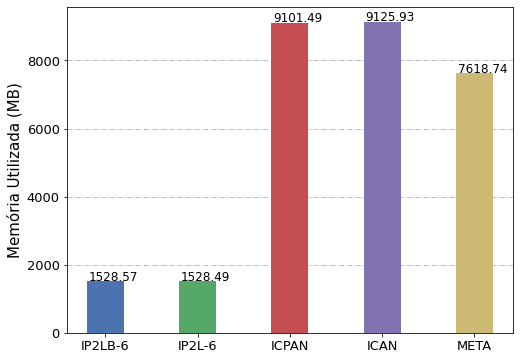
\includegraphics[width=0.8\textwidth]{figures/memory_usage_baselines_dataset_usaddr_tau_3.png}
    \caption{Gráfico de barras para as quantidades de memória em \textit{MegaBytes} utilizada por cada método, considerando $\lambda = 6$ para os métodos IP2LB e IP2L.}
    \label{fig:memory-usage-baselines-usaddr-tau-3}
\end{figure} 

\cleardoublepage
